% --------------------------------------------------------------------------
% Template for DCASE 2018 paper; to be used with:
%          dcase2018.sty  - DCASE 2018 LaTeX style file, and
%          IEEEbib.bst - IEEE bibliography style file.
% Adapted from spconf.sty and waspaa15.sty
% --------------------------------------------------------------------------

\documentclass{article}
\usepackage{dcase2018,amsmath,graphicx,url,times,booktabs, tabularx}
\usepackage{bbm}
% Example definitions.
% --------------------
\def\defeqn{\stackrel{\triangle}{=}}
\newcommand{\symvec}[1]{{\mbox{\boldmath $#1$}}}
\newcommand{\symmat}[1]{{\mbox{\boldmath $#1$}}}

% Title.
% --------------------
\title{Towards perceptual soundscape characterization using event detection algorithms}
     
\name{F\'elix Gontier$^{1}$,
       Mathieu Lagrange$^{1}$,
       Jean-Francois Petiot$^{1}$
       }
 \secondlinename{	  
       Catherine Lavandier$^{2}$,
       Pierre Aumond$^{3}$
       }
       % fixed *.sty to allow names on multiple lines
 \address{$^1$ LS2N, UMR 6004, Ecole Centrale de Nantes, CNRS, 44322 Nantes, France, \{felix.gontier\}@ls2n.fr\\          
         $^2$ ETIS, UMR 8051, Universit\'e Paris Seine, Universit\'e de Cergy-Pontoise, ENSEA, CNRS, \\ 95000 Cergy-Pontoise, France, \{catherine.lavandier\}@u-cergy.fr\\ 
         $^3$ UMRAE, Ifsttar, 44341 Bouguenais, France, 
         \{pierre.aumond\}@ifsttar.fr\\
  }

\begin{document}

\ninept
\maketitle

\begin{sloppy}

\begin{abstract}

\end{abstract}

\begin{keywords}
\end{keywords}

%TODO : Abstract
%TODO : Finish intro
%TODO : Finish discussion
%TODO : Bibliography & refs

\section{Introduction}
\label{sec:intro}

The ongoing urbanization process has led to an increase in sound quality concerns. In urban areas the noise has been linked to several health issues including sleep-related troubles as well as heart diseases rates, and is a major cause for city dwellers' annoyance in certain areas. In this context, the 2002/49/CE European directive (CITE) requires that large cities maintain noise maps to facilitate the development of noise reducing plans. These noise maps are mainly based on predictive and propagation models. The studies are often limited to traffic and other transportation sources few physical measurements are used. Furthermore, the models depend on topological data that may be unavailable or undercomplete. The advent of the Internet of Things (IoT) presents an opportunity for the development of large, scalable networks of acoustic sensors. The Characterization of Urban Sound Environments (CENSE) project (CITE) aims at implementing such a network to produce perceptually motivated noise maps.

Introducing perception-related notions such as liveliness or familiarity is necessary to assess the quality of urban soundscapes (CITE). The study of relevant feelings describing the appreciation of soundscapes results in the mapping of perceptual spaces (CITE) which are used as a basis for perceptual experiments. The dimension of pleasantness is increasingly associated with soundscape quality in recent works (CITE).

The traditionally used energetic (sound levels, eg. $L_{Aeq}$) and psychoacoustic (eg. Zwicker's loudness $N$) indicators are not considered sufficient to characterize the perception of a sound scene (CITE). Soundscape pleasantness is on the contrary highly dependent on the composition of the scene (CITE) as each sound source has a different impact, for example the soundscape quality is likely to be improved by birdsongs and deteriorated by construction noises. Several proposals on sets of relevant indicators (CITE) have been published to better account for the specificities of each scene. Though, the established metrics are mostly derived from physical measurements on longer durations or added information such as traffic flow density.

The use of large-scale sensor networks yields a problematic for the extraction of content-related quantities of interest from important amounts of data. Despite a growing interest in the community, machine learning models - to the best of our knowledge - were not successfully applied to the prediction of source-specific perceptual parameters in complex urban environments. Most event detection applications focus on obtaining a precise localization of source activity, within usual ranges of tens of milliseconds. Source separation models are trained to output the closest estimates to the ground truth. In that regard, predicting the perceived pleasantness is a middle ground. Both detection and level estimation are necessary although perceptual notions are evaluated on longer time scales. The ground truth characteristics of a sound event in a complex scene are likely not to be captured by human perception, as well as differ individually.

Nevertheless, several tools and resources have been proposed to approach soundscape characterization as a machine learning problem. The Sounds of New-York City (SONYC) project (CITE) released the UrbanSound (CITE) and Urban-Sed (CITE) datasets for sound event classification and detection in urban environments respectively. Sound scene synthesis libraries such as simScene (CITE) and Scaper (CITE) also palliate the difficulty of constructing corpora dedicated to a specific task. Large datasets can be created in a controlled manner to cover experimental plans while providing ground truth information without the need of human annotation.

Challenges such as Detection and Classification of Acoustic Scenes and Events (DCASE) are proposed to apply complex detection and classification models to real-life data and applications in the urban context. This involves soundscape categorization and sound event detection with added difficulties (weak labeling, rare events). The objective of this work is to formally propose a task based on sound event detection and classification for the perceptual characterization of sound scenes in a urban environment.

\clearpage

\section{Characterization Task}
\label{sec:char}
Several perceptual studies of the urban soundscape quality have been led to propose a model of pleasantness from other perceptual parameters (CITE). In all cases, a good approximation of pleasantness can be obtained by linear combination of both overall and source-specific parameters: 
\begin{equation}
P = aL + \sum_s b_sT_s + c
\end{equation}
where $T_s$ is the perceived time presence for source $s$. The coefficients $a$, $b_s$ and $c$ are usually found via multiple linear regression and thus differ in each study.
Furthermore, three principal source categories are identified: mechanical, human and animal. Mechanical sounds are mainly composed of traffic and have a negative impact on soundscape pleasantness. Animal sources (bird activity) have a positive influence while human sounds (voices) can yield mixed effects.

Given these models, the prediction of pleasantness can be assimilated as that of perceived time presences. These quantities of interest are more closely related to the audio signal and their assessment represents a fitting application for detection models proposed in the data science and machine learning community. We thus introduce a new detection and classification task proposal. The dataset for this task is a collection of one minute long simulated sound scenes created using simScene (CITE) or Scaper (CITE). The use of simulated scenes offers multiple advantages: their composition and complexity is entirely controllable and source-specific channels can be accessed with ground truth annotations. Considering the models proposed in the litterature the taxonomy for sources of interest is limited to traffic, voice and bird activities. Multiple environments are also considered for compositional variability: park, quiet street, noisy street, very noisy street and square. Finally, the development part of the dataset is published with the corresponding separated tracks for each source, the evaluation dataset only contains mixed scenes.

Three levels of metrics are identified for this task. First, the physical level is evaluated with a 125~ms precision on the presence and emergence of the three sound sources. The presence is a binary value and the emergence is chosen as a five-point scale (Not heard - Dominant) rather than as a sound level. The motivation for this choice is two-fold: discrete scales are suficient when the metric is linked to perceptual parameters, and the problem is translated from source separation and estimation to classification. The second level is the perceived time presence for each source in the whole scene represented as a scalar in the 0-1 range. The third level is the estimate of pleasantness over the scene, also represented as a 0-1 scalar. The transition models from one level to the next are known and published. As a result and because our interest is focused on pleasantness, models can be designed to predict the metrics at either level.

\section{Perceptual validation}
\label{sec:val}

We conduct a perceptual experiment to validate the proposed characterization task. Its objectives are to study the relation between extracted source-dependant physical indicators to their perceptual equivalents, then confirm the relevance of the first level of metrics described in Section~\ref{sec:char}.

For this perceptual test, we use a set of sound scenes recorded in the 13th district of Paris as part of the GRAFIC project (CITE). Of the 19 different recording locations, 9 are selected to represent diverse compositional properties: park (P3, P9), quiet street (P5, P11, P13, P17), noisy street (P2, P6) and very noisy street (P16).

The scenes are re-simulated (CITE) using the Matlab toolbox \textit{simScene} (CITE). First, the sound extracts are annotated by ear by identifying active background and event sources. Background sounds are present throughout the whole scene and are characterized by a SNR parameter. Conversely, events are localized occurences that are defined by their start and end times as well as an event-to-background ratio (EBR). The sound scenes are simulated from these annotations and a database of extracts for isolated sources. This ensures access to separated channels from which ground truth source-specific presence and sound level can be computed. One minute of audio is finally extracted for each scene such as no single event overwhelms the perception of the rest of the excerpt. 

During the test, the order of appearance is as follows: the scenes from locations P3 and P16 representing very quiet (park) and very noisy (very noisy street) environments are always presented first to calibrate the subject's answers. The remaining sounds are presented in random order to limit order biases over the participants population. For each scene, 14 criteria are evaluated on a 0-10 scale by the subject. The first four questions cover general sound level and perceptual parameters:
\begin{enumerate}
\item \textit{Bruyant - Silencieux}: Overall perceived loudness (OL),
\item \textit{Ennuyeux, inint\'eressant - Stimulant, int\'eressant}: Interest (I),
\item \textit{Inerte, amorphe - Anim\'e, mouvement\'e}: Liveliness (L),
\item \textit{Agit\'e, chaotique - Calme, tranquille}: Calmness (C).
\end{enumerate}
Source-specific perceived time presence (scale \textit{Jamais - Continuellement}) and sound level (scale \textit{Tr\`es faible - Tr\`es fort}) are also evaluated. The considered sources are traffic (T), birds (B), horns and sirens (H), human voice (V) and footsteps (F). Perceived time presence and level for source S are respectively noted S\_T and S\_L in the remainder of this paper.

The test is conducted using a Python interface. Participants can only listen once to each scene and must answer all questions before proceeding to the next extract. All subjects used the same desktop configuration, sound card and software, as well as Beyerdynamics DT-990 headphones in a quiet environment. The same sound output level was set by the experimenter for all scenes and participants. 30 subjects took the test in 3 sessions, all reported normal hearing conditions.

An outlier detection procedure is applied on the 270 resulting assessments (30 subjects, 9 scenes). An assessment is rejected when it is located away from the mean by more than 3 standard deviations at the question level, that is for each parameter of each scene. The results from two participants with more than 10\% assessments considered as outliers are removed from the study, which thus includes 252 individual assessments on 20 parameters.

The perceptual space produced by the test is first compared to previous studies in the litterature (CITE). This is to ensure that relevant conclusions can be made on further analysis. Figure~\ref{fig:pca} shows the principal components analysis (PCA) of the four general questions at the assessment level. The first two components explain 52.3\% and 30.5\% of the global variance respectively. It is found that liveliness (L) correlates poorly with calmness (C), while interest (I) is between the two. These results can be compared to previous studies on similar pleasantness parameters~\cite{axelsson2010,jeon2018}, where interest and calmness were established as almost independant. The scale of liveliness was in both cases correlated similarly with the the two others. However, just as the principal components space was slightly distorted in~\cite{jeon2018} due to the study being focused on park environments, here the small size of the considered corpus in terms of number of scenes also affect the relations between perceptual parameters. The absence of a dedicated pleasantness scale in our study limits further comparisons.

\begin{figure}[t]
  \centering
  \centerline{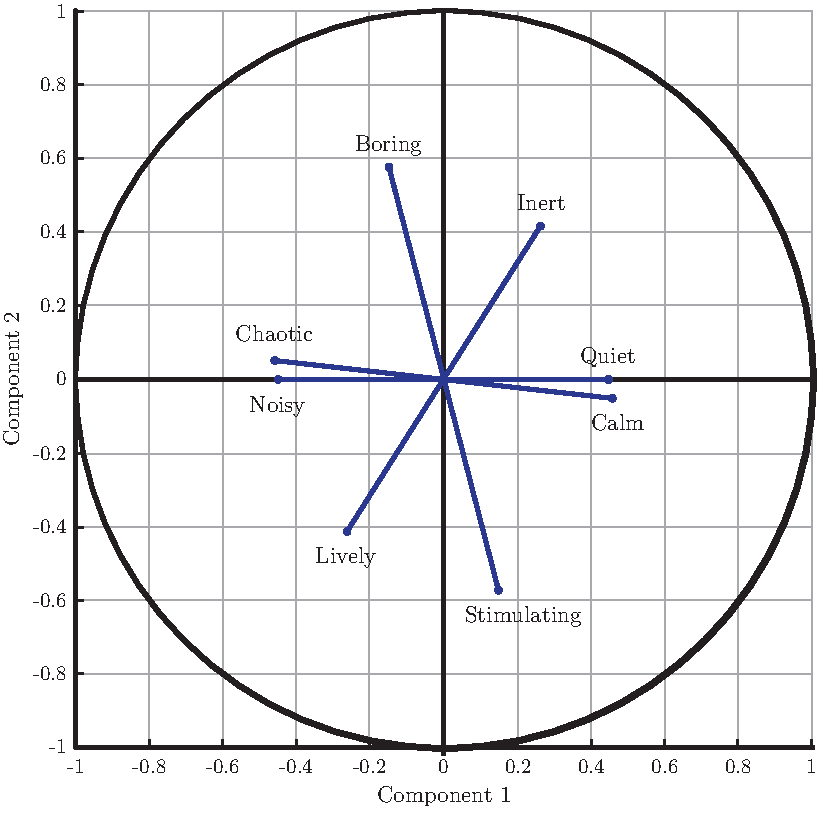
\includegraphics[width=\columnwidth]{pca.pdf}}
  \caption{Principal component analysis (first two components) of the four general perceptual parameters at the scene level (n=9). }
  \label{fig:pca}
\end{figure}

The main objective of this work is to predict pleasantness parameters from acoustical data without perceptual assessments. As shown in Section~\ref{sec:char} several models have been established to assess pleasantness as a function of perceived sound sources. Thus, physical indicators are computed from the audio tracks obtained during scene simulation. To evaluate the overall loudness of the scene three measurements are chosen in accordance with the litterature (CITE):
\begin{itemize}
\item L50: Z-weighted (no weighting over the observed frequency range) sound level exceeded 50\% of the time in dB,
\item LA50: A-weighted sound level exceeded 50\% of the time in dBA,
\item L50 for the 1kHz band only.
\end{itemize}
The time-frequency second derivative (TFSD) indicator was shown to improve pleasantness predictions in \cite{aumond}. Two TFSD indicators are computed: the TFSD at $4~kHz$ and $125~ms$ frame length which is found to strongly correlate with the perceived bird presence, and at $500~Hz$ and $1~s$ frame length which correlates with human voice presence.

\begin{table*}[ht!]
\centering
\caption{Pearson correlation coefficients between perceptual parameters and physical indicators at the scene level (n=9). *: $p<0.05$, **: $p<0.01$, non-significant correlations ($p>0.05$) are noted NS.}
\label{table:pearsonc}
\resizebox{2\columnwidth}{!}{
\begin{tabular}{ l | c c c c c c c c c c c c c c }
\hline
	Phys./Perc. & OL & I & L & C & T\_L & T\_T & B\_L & B\_T & H\_L & H\_T & V\_L & V\_T & F\_L & F\_T \\ \hline
	$L50_{1kHz}$ & 0.93** & NS & NS & -0.92** & 0.75* & 0.7* & NS & NS & NS & NS & NS & NS & NS & NS \\
	$L50$ & 0.98** & NS & 0.73* & -0.97** & 0.72* & NS & NS & NS & NS & NS & NS & NS & NS & NS \\
	$LA50$ & 0.96** & NS & 0.73* & -0.94** & NS & NS & NS & NS & NS & NS & NS & NS & NS & NS \\ \hline
	$TFSD_{500Hz}$ & NS & NS & NS & NS & NS & NS & NS & NS & NS & NS & NS & NS & NS & NS \\
	$TFSD_{4kHz}$ & NS & 0.88** & NS & NS & -0.72* & -0.71* & 0.92** & 0.81** & NS & NS & NS & NS & NS & NS \\ \hline
	$T_T$ & NS & NS & NS & NS & NS & NS & NS & NS & NS & NS & NS & NS & NS & NS \\
	$T_L$ & NS & NS & NS & NS & NS & NS & NS & NS & NS & NS & NS & NS & NS & NS \\ \hline
	$B_T$ & NS & 0.67* & NS & NS & 0.71* & 0.75* & NS & NS & NS & NS & NS & NS & NS & NS \\
	$B_L$ & NS & 0.93** & NS & NS & -0.84** & -0.83** & 0.91** & 0.82** & NS & NS & NS & NS & NS & NS \\ \hline
	$H_T$ & NS & NS & NS & NS & NS & NS & NS & NS & NS & 0.84** & NS & NS & NS & NS \\
	$H_L$ & NS & NS & NS & NS & NS & NS & NS & NS & 0.98** & 0.78* & NS & NS & NS & NS \\ \hline
	$V_T$ & NS & NS & NS & NS & NS & NS & NS & NS & NS & NS & NS & NS & NS & NS \\
	$V_L$ & NS & NS & 0.81** & NS & NS & NS & NS & NS & NS & NS & 0.84** & 0.88** & NS & NS \\ \hline
	$F_T$ & NS & NS & NS & NS & NS & NS & NS & NS & NS & NS & NS & NS & 0.9** & 0.68* \\
	$F_L$ & NS & NS & -0.72* & NS & NS & NS & NS & NS & NS & NS & -0.69* & -0.78* & 0.92** & NS \\ \hline
	$T_T(\alpha)$ & NS & -0.81** & NS & NS & 0.90** & 0.94** & NS & NS & NS & NS & NS & NS & NS & NS \\
	$T_T(\alpha, \beta)$ & NS & -0.80** & NS & NS & 0.88** & 0.92** & NS & NS & NS & NS & NS & NS & NS & NS \\ \hline
	$T_B(\alpha)$ & NS & 0.88** & NS & NS & NS & NS & 0.95** & 0.97** & NS & NS & NS & NS & NS & NS \\
	$T_B(\alpha, \beta)$ & NS & 0.88** & NS & NS & NS & NS & 0.95** & 0.97** & NS & NS & NS & NS & NS & NS \\ \hline
	$T_H(\alpha)$ & NS & NS & NS & NS & NS & NS & NS & NS & NS & 0.83** & NS & NS & NS & NS \\
	$T_H(\alpha, \beta)$ & NS & NS & NS & NS & NS & NS & NS & NS & 0.73* & 0.88** & NS & NS & NS & NS \\ \hline
	$T_V(\alpha)$ & NS & NS & 0.82** & NS & NS & NS & NS & NS & NS & NS & 0.79* & 0.83** & NS & NS \\
	$T_V(\alpha, \beta)$ & NS & NS & 0.82** & NS & NS & NS & NS & NS & NS & NS & 0.75* & 0.79* & NS & NS \\ \hline
	$T_F(\alpha)$ & NS & NS & NS & NS & NS & NS & NS & NS & NS & NS & NS & -0.71* & 0.87** & NS \\
	$T_F(\alpha, \beta)$ & NS & NS & NS & NS & NS & NS & NS & NS & NS & NS & NS & NS & 0.90** & 0.70* \\ \hline
\end{tabular}
}
\end{table*}

Source-specific indicators are also computed: the time presence and an emergence estimation, obtained by subtracting the global L90 (Z-weighted level exceeded 90\% of the time) found to represent well background activity to the L10 of each source (CITE). The emergence is considered for the whole source activity while time presence can only be associated to sound events. Furthermore, all sound levels are computed with the Matlab ITA toolbox (CITE) in the 20~Hz-20~kHz range.

In the considered scenes, background sources are always active. The measurement of time presence is thus limited to sound events which leads to poor correspondance with perceptual responses. This is particularly visible for traffic sources, on which most pleasantness parameters strongly depend. While being objectively present over the whole duration of the scenes, traffic is not perceived as such in quiet scenes (park, quiet street). Furthermore, the proposed indicators only consider each sound source separately, not taking into account potential masking effects by other sources active at the same time. Two additional indicators are thus proposed regarding these considerations.



The first proposed indicator $T_s(\alpha)$ relies on the emergence of each sound source relative to the others over time. Sound levels (dB SPL) are computed for audio frames of 125~ms. This duration approximately corresponds to that of the shortest found event and is widely used in acoustical monitoring applications. The emergence, \textit{i.e.} difference $\Delta_s(t)$ of sound levels between the studied source ($L_s(t)$) and the background ($L_b(t)$) is computed. No difference is made between background and event sources. The source is then considered present on a given frame if the emergence is greater than a threshold value $\alpha$. Finally, a time presence measurement is obtained by averaging over time:
\begin{equation}
T_s(\alpha) = \frac{1}{N_t}\sum_{t = 1}^{N_t}\mathbbm{1}_{\Delta_s(t)>\alpha}
\end{equation}
where $N_t$ is the total number of 125~ms analysis frames in the scene. The optimal threshold is found via grid search to be $\alpha = -31dB$ for the considered corpus. If a source is objectively present it will almost always considered present regardless of the other contents of the scene.

However, the masking of a sound by another does not depend only on the emergence over the whole frequency spectrum. The spectral composition is important: in a signal with a monophonic tone and large band noise, the noise has to be at a higher level to mask completely the tone. The level comparison must be made around the fundamental frequency of the tone. A second indicator $T_s(\alpha, \beta)$ is thus proposed. Third-octave bands sound levels are computed on 125~ms frames and the emergence of a source compared to the background is defined as
\begin{equation}
\Delta_s(t, f) = L_s(t, f) - L_b(t, f)
\end{equation}
Similarly to the first metric $T_s(\alpha, \beta)$ then relies on simple thresholds applied on the emergence, first in frequency then in time. Its expression is as follows:
\begin{equation}
T_s(\alpha, \beta) = \frac{1}{N_t}\sum_{t = 1}^{N_t}\mathbbm{1}\left[ \frac{\sum_{f = 1}^{N_f}\Delta_s(t, f)\mathbbm{1}_{\Delta_s(t, f)>\alpha}}{\sum_{f = 1}^{N_f}\mathbbm{1}_{\Delta_s(t, f)>\alpha}}>\beta \right]
\end{equation}
where $N_f$ is the number of third-octave bands. Again, optimal values for parameters $\alpha_{opt} = -6 dB$ and $\beta_{opt} = -5 dB$ are found via grid search. This is a much more plausible set of values, indicating that a source's emergent frequency components must be on average at most 5~dB less than other sources present at the same time for the source to be heard.


Table~\ref{table:pearsonc} shows the Pearson's correlation coefficients between the computed indicators and assessed parameters at the sound scene level. Global sound levels represent very well the perceived overall loudness of the scene. The $TFSD_{500Hz}$ is not significantly correlated to the perception of human voices, and the $TFSD_{4kHz}$ does not discriminate parameters related to traffic and bird presence. Ground truth indicators suffer from similar problems. Traffic is almost always present in the background of the studied soundscapes but can be masked by other sources. As a result the ground truth time presence and emergence are not efficient when used separately to characterize perception of traffic. The two proposed emergence-based time presence indicators achieve better performances: they are discriminative and show high correlations with the perception of corresponding sources.


\section{Discussion}
\label{sec:disc}

We presented a pilot experiment to assess the feasability of the prediction of perceptual parameters from acoustic indicators in simulated scenes. 

As expected, the physical time presence of sources is not sufficient to fully characterize soundscape perception. The proposed indicator $T_s(\alpha, \beta)$, while relying on a simple emergence model due to the small amount of available data, can be directly linked to source-specific perceptual quantities. It is notably more efficient for the assessment of traffic activity, which is heavily present in the background of sound scenes in a urban context. This illustrates the need to account for emergence of sources as a metric to determine their perceptual importance in complex sound scenes. Predicting the average pleasantness of a soundscape can thus be achieved by estimating the source activity and emergence indicators proposed in Section~\ref{sec:char}. 

The postulated precision requirements of estimates are also confirmed. All physical indicators in the presented experiment are computed at a 125~ms or longer time scale, and show strong relations to perceptual evaluations. A binary masking model is used in this study that improves parameter predictions. The estimation of source-wise emergence as a classification process on a 5-point scale as opposed to regression is thus considered sufficient for the application needs.

For all sources the perceived time presence and sound level are highly correlated ($r>0.8, p<0.01$). This is not the case for the corresponding acoustical indicators indicating information redundance between these two quantities at the perceptual level. The sound level can thus be omitted in the pleasantness model. Furthermore, multiple linear regressions confirm that sources beside traffic, voices and birds have little impact on the observed perceptual notions of interest, liveliness and calmness. Energetic indicators such as the $L_{50}$ are closely related to overall sound level perception and no additional prediction is required as part of the task.

Future work includes a second, more complete test specifically designed to cover the experimental plan induced by this task proposal. Its primary objective is to propose a definitive model linking physical indicators to perceptual quantities. For this experiment, a corpus should be built observing the taxonomies proposed in Section~\ref{sec:char} in terms of environments and sources. Furthermore, it should study the validity of existing pleasantness models for simulated scenes.



% -------------------------------------------------------------------------
% Either list references using the bibliography style file IEEEtran.bst
\bibliographystyle{IEEEtran}
\bibliography{refs}
%
% or list them by yourself
% \begin{thebibliography}{9}
% 
% \bibitem{dcase2016web}
%   \url{http://www.cs.tut.fi/sgn/arg/dcase2016/}.
%
% \bibitem{IEEEPDFSpec}
%   {PDF} specification for {IEEE} {X}plore$^{\textregistered}$,
%   \url{http://www.ieee.org/portal/cms_docs/pubs/confstandards/pdfs/IEEE-PDF-SpecV401.pdf}.
%
% \bibitem{PDFOpenSourceTools}
%   Creating high resolution {PDF} files for book production with 
%   open source tools, 
%   \url{http://www.grassbook.org/neteler/highres_pdf.html}.
%
% \bibitem{eWilliams1999}
% E. Williams, \emph{Fourier Acoustics: Sound Radiation and Nearfield Acoustic
%   Holography}. London, UK: Academic Press, 1999.
% 
% \bibitem{ieeecopyright}
%   \url{http://www.ieee.org/web/publications/rights/copyrightmain.html}.
%
% \bibitem{cJones2003}
% C. Jones, A. Smith, and E. Roberts, ``A sample paper in conference
%   proceedings,'' in \emph{Proc. IEEE ICASSP}, vol. II, 2003, pp. 803--806.
% 
% \bibitem{aSmith2000}
% A. Smith, C. Jones, and E. Roberts, ``A sample paper in journals,'' 
%   \emph{IEEE Trans. Signal Process.}, vol. 62, pp. 291--294, Jan. 2000.
% 
% \end{thebibliography}


\end{sloppy}
\end{document}
